\documentclass{article}
\usepackage{protools}
\setlength\parskip{0.25\baselineskip}

\addbibresource{towards.bib}

\begin{document}

\ArticleTitle
  {Towards Optical States Of Four Photons}
\ArticleAuthor*
  [0000-0002-5646-6964]
  {Jan Provazn\'{i}k}
  {provaznik@optics.upol.cz}
\ArticleAuthorAddress
  {Department of Optics, Palack\'{y} University, 17. listopadu 1192/12, 771 46 Olomouc, Czech Republic}

\ArticleAuthor
  {Olga Solodovnikova}
\ArticleAuthorAddress
  {Technical University of Denmark, Lyngby, Denmark}

\ArticleAuthor
  [0000-0002-5761-8966]
  {Petr Marek}
\ArticleAuthorAddress
  {Department of Optics, Palack\'{y} University, 17. listopadu 1192/12, 771 46 Olomouc, Czech Republic}

\ArticleAuthor
  [0000-0003-4114-6068]
  {Radim Filip}
\ArticleAuthorAddress
  {Department of Optics, Palack\'{y} University, 17. listopadu 1192/12, 771 46 Olomouc, Czech Republic}

\ArticleTitlePrint

\begin{abstract}\noindent
  Quantum non-Gaussian states of traveling light fields are crucial components of quantum information processing protocols; however, their production is experimentally challenging. In this paper, we discuss the minimal requirements imposed on the quantum efficiency of photon number resolving detectors and the quality of the squeezing operation in an experimental realization of certifiable quantum non-Gaussian states of individual photonic states with three, four, and five photons.
\end{abstract}

% Introduction
%

\section{Introduction}

Quantum non-Gaussian states of traveling light fields are the lifeblood of scalable fault-tolerant quantum computation protocols employing continuous-variable quantum systems~\cite{lloyd1999,gottesman2001,menicucci2014,baragiola2019,bourassa2021,madsen2022,aghaeerad2025}. Unfortunately the production of these states is experimentally challenging due to the scarcity of naturally occurring non-Gaussian interactions.

The lack of physical non-Gaussian interactions can be resolved with measurement-induced operations~\cite{filip2005,marek2009,marek2011,yukawa2013b,miyata2016,marek2018a,sakaguchi2023}, which can be implemented using Gaussian interactions and appropriate ancillary non-Gaussian states. The bespoke non-Gaussian ancillaries can be tailored precisely to their purpose and synthesized with several methods, for example, by utilizing photon addition and subtraction~\cite{dakna1999,fiurasek2005,eaton2019,takase2021,endo2023}, manipulating and measuring entangled states~\cite{yukawa2013a,yoshikawa2018,tiedau2019,provaznik2020}, and exploiting Gaussian boson samplers~\cite{su2019,quesada2019}. Intricate breeding protocols can also be employed to produce more complex non-Gaussian states~\cite{weigand2018,eaton2022,zheng2023,takase2024,aghaeerad2025}. % It is not possible to concoct non-Gaussianity without actual non-Gaussian resources~\cite{walschaers2021}. These can be facilitated by, for example, photon number resolving (PNR) detectors.

So far, only superpositions of up to three photons have been crafted as realistic approximations of cubic phase states using a two-mode squeezed vacuum, displacement operations, and appropriate heralding~\cite{yukawa2013a,yukawa2013b}. This method can be principally adapted to prepare superpositions of higher Fock states. The experimental capacity to prepare more complicated superpositions can be demonstrated by first constructing individual states with four photons. Their preparation requires far looser experimental control, as no additional operations are involved beyond the initial two-mode squeezed vacuum state and a photon number resolving detector used for heralding. Nonetheless, it still relies on high-quality noiseless squeezing and efficient detection.

The omnipresent loss in realistic experiments negatively affects the prepared states. Under these conditions, the desired four-photon states can not be prepared faithfully. Their quality can not be reliably assessed using fidelity; this measure makes sense only for states close to their ideal counterparts. Instead, the state can be characterized by its stellar rank, a property that can not be increased by Gaussian means, including loss and Gaussian noise~\cite{walschaers2021}. The quality of the state can be certified using a stellar rank witness based on the hierarchical quantum non-Gaussian criteria~\cite{lachman2019,fiurasek2022}.

In this paper, we discuss the minimal requirements imposed on the quantum efficiency of photon number resolving detectors and the quality of the squeezing operation in an experimental realization of certifiable quantum non-Gaussian states of individual photonic states with three, four, and five photons.

This document comprises two primary sections:  methodology and discussion of the findings. The first section introduces a mathematical model of the measurement-based photonic circuit capable of preparing individual photonic states of light, discusses the hierarchical criteria used to certify genuine quantum non-Gaussian states, and describes the Monte Carlo simulation of the experiment and the subsequent interpretation of its results. Figures presented in the second section determine the minimal requirements for the efficiency of the optical components, such as squeezing and detection, in experimental realizations targeting states of three, four, and five photons.

% A measurement-based method for preparation of individual photonic states of light~\cite{yukawa2013a,yoshikawa2018,tiedau2019,provaznik2020} is discussed in the first section of this chapter. The mathematical model of the procedure takes loss into account, both in the construction of the state in during its characterization. The resulting states are certified using hierarchical criteria~\cite{lachman2019} in the second section by evaluating the statistical behavior of the model under realistic experimental conditions. Figures presented in this section can be used to determine the minimal requirements on the efficiency of the optical components, such as squeezing and detection, in experimental realizations targeting states of two, three, and four photons.

% Methodology
%

\section{Cooking up states of travelling light}

Photonic Fock states can be conditionally prepared using a two-mode squeezed vacuum state and a photon number resolving detector~\cite{yukawa2013a,yoshikawa2018,tiedau2019,provaznik2020}. The theoretical model of the experimental scheme is illustrated in~\figref{f-scheme}. One of the entangled modes is measured, thus projecting the other mode onto the resolved Fock state. This procedure is repeated until a satisfactory detection outcome in the heralding mode is observed; at this point, the target state is successfully prepared. In the case of an unfavorable detection event, the state is discarded, and the whole procedure is repeated.

\begin{figure}[h]
  \begin{center}
    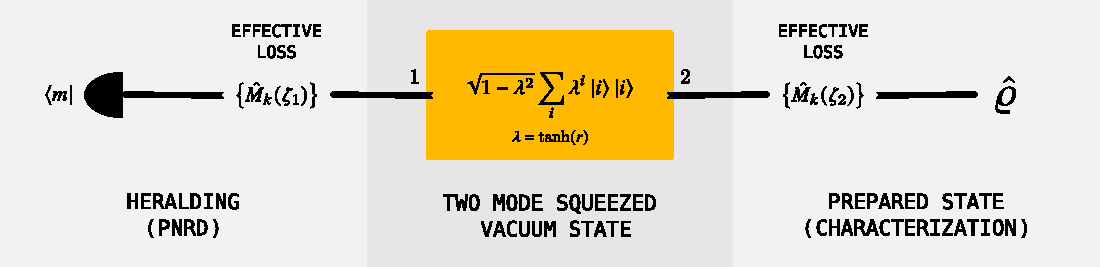
\includegraphics[width = 1.00 \columnwidth]{import/illustrate_scheme_alt.pdf}
  \end{center}
  \caption{
    Schematic illustration of the non-Gaussian state preparation circuit with a two mode squeezed vacuum state serving as a source of entangled quantum states. One of the modes is measured, thus projecting the other mode onto the resolved Fock state. 
  }
  \label{f-scheme}
\end{figure}

One of the principal experimental challenges in preparing quantum states of light is the omnipresent loss and noise. It diminishes quantum correlations between entangled resources and reduces the quantum efficiency of detectors, making it impossible to prepare the desired quantum state with perfect fidelity. The reduced detection efficiency negatively affects the preparation of the quantum state and its subsequent characterization. The procedure outlined in~\figref{f-scheme} assumes a perfectly squeezed state and an ideal photon number resolving (PNR) detector. The adverse effects of realistic inefficiencies can be accounted for by considering a lossy transmission of both modes prior to their measurement with ideal detectors~\cite{feito2009}.

The resulting non-normalized marginal state is given by
%
\begin{equation}\label{e-pnr-rho}
  \hatrho_{(m)} \approx
  \sum_{i = 0}^{\infty} 
  \sum_{j = 0}^{\infty}
    \lambda^{i} \lambda^{j}
    \left(
      \sum_{k = 0}^{\infty}
        \bra{m} \hat{M}_{k} (\zeta_{1}) \ketbra{i}{j} \hat{M}_{k}^{\dagger} (\zeta_{1}) \ket{m}
    \right)
    \left(
      \sum_{k = 0}^{\infty}
        \hat{M}_{k}(\zeta_{2}) \ketbra{i}{j} \hat{M}_{k}^{\dagger} (\zeta_{2})
    \right) \Qc
\end{equation}
%
where~$m$ identifies the detected Fock state,~${\lambda = \tanh(r)}$ characterizes the two-mode squeezed state with initial squeezing~$r$, and the Kraus operators~${\hat{M}_{k} (\zeta)}$ describe the transmission loss with
%
\begin{equation}
  \hat{M}_{k} (\zeta) =
    \sqrt{ \frac{(1 - \zeta)^{k}}{k!} } 
    \sqrt{\zeta}^{\hat{n}} \hat{a}^{k}
\end{equation}
%
where~$\zeta$ gives the intensity transmittance of the lossy channel~\cite{ivan2011}. In the case of~\eqref{e-pnr-rho}, the parameter~$\zeta_{1}$ corresponds to the loss in the first mode, called the heralding mode, whereas~$\zeta_{2}$ describes the loss affecting the mode carrying the prepared state.

The probability of successful preparation, that is, the probability of detecting~$m$ photons in the heralding mode, can be obtained analytically as
%
\begin{equation}\label{e-pnr-pro}
  P_{(m)} = (1 - \lambda^{2}) 
  \frac
    { (\lambda^{2} \zeta_{1})^{m} }
    { [ 1 - \lambda^{2} (1 - \zeta_{1}) ]^{m + 1} } \Qd
\end{equation}
%
The equation~\eqref{e-pnr-rho} for the resulting density matrix of the prepared state can be simplified. The matrix is diagonal in the Fock basis; its properly normalized elements are obtained as
%
\begin{equation}\label{e-pnr-rho-kk}
  \braket{ k | \hatrho_{(m)} | k } =
  \frac
    { [ 1 - \lambda^{2} (1 - \zeta_{1}) ]^{m + 1} }
    { [ \lambda^{2} (1 - \zeta_{1}) ]^{m} }
  \left( \frac{ \zeta_{2} }{ 1 - \zeta_{2} } \right)^{k}
  H (k, m, x) \Qc
\end{equation}
%
where the substitution~${x \coloneqq \lambda^{2} ( 1 - \zeta_{1} )(1 - \zeta_{2} )}$ is used in the function~$H(k, m, x)$ defined as
%
\begin{equation}\label{e-H}
  H(k, m, x) \coloneq
  \sum\limits_{l = \tau_{km}}^{\infty}
    \binom{l}{m}
    \binom{l}{k}
    x^{l} 
\end{equation}
%
with~${\tau_{km} \coloneqq \max(k, m)}$. The infinite series in~\eqref{e-H} is convergent as the substituted argument $x$ satisfies~${\abs{x} \leq 1}$. It can be equivalently expressed using a suitable hypergeometric function~\cite{bateman1981}
%
\begin{equation}
  \begin{aligned}
    H(k, m, x) & =
    x^{\tau_{mk}} 
    \binom
      {\tau_{mk}}
      {\kappa_{mk}}
    {}_{2}F_{1} (
      1 + \tau_{mk},
      1 + \tau_{mk},
      1 + \tau_{mk} - \kappa_{mk},
      x
    ) \\
    & =
    x^{\tau_{mk}} F(k, m, x),
  \end{aligned}
\end{equation}
%
where ${\kappa_{mk} \coloneqq \min (m, k)}$. The hypergeometric function can be evaluated with the help of commonly available numerical libraries~\cite{virtanen2020}. 

The formula \eqref{e-pnr-rho-kk} deserves further discussion. The first two fractions seemingly diverge in the ideal lossless cases when either ${\zeta_{1} \to 1}$ or ${\zeta_{2} \to 1}$. It may also diverge if there is no initial two-mode squeezing applied, that is, when ${\lambda \to 0}$. The offending elements can be propagated into the $H(k, m, x)$ function, leading to the full expression
%
\begin{equation}
  { [ 1 - \lambda^{2} (1 - \zeta_{1}) ]^{m + 1} }
  { \zeta_{2}^{k} }
  \left(
    \lambda^{2 (\tau_{mk} - m)}
    (1 - \zeta_{1})^{\tau_{mk} - m}
    (1 - \zeta_{2})^{\tau_{mk} - k}
  \right)
  F (k, m, x),
\end{equation}
%
where both ${\tau_{mk} - m \geq 0}$ and ${\tau_{mk} - k \geq 0}$ in the potentially diverging powers of the ${1 - \zeta_{1}}$, ${1 - \zeta_{2}}$ and $\lambda^{2}$ coefficients.

\subsection*{Approximate photon number resolving detectors}

The model of state preparation, represented by relation~\eqref{e-pnr-rho}, relies on true PNR detectors in the heralding stage of the circuit. While these detectors exist in principle~\cite{hopker2019,endo2021,endo2024}, their practical availability is severely limited. The model of the experimental circuit can be extended to cover the more commonly available cascaded avalanche photodiode (CAP) detectors~\cite{hlousek2019,grygar2022,hlousek2024,ercolano2024} that operate by dividing the incoming signal equally between~$n$ independent avalanche photodiode detectors and counting the number~$m$ of detectors that registered photons. The avalanche detectors can only distinguish between zero and non-zero numbers of incident photons; this hinders the possibility of photon number resolution by the cascade. It approximates true PNR detectors well only in the limit of large numbers~$n$ of the constituent avalanche detectors~\cite{provaznik2020}. The detection events when~$m$ out of the $n$ detectors register photons are associated with the operators~\cite{paul1996}
%
\begin{equation}\label{e-cap}
  \begin{gathered}
  \hat{\Pi}_{m}^{n} 
    \coloneqq \sum_{i = 0}^{\infty} w(i, m, n) \ketbra{i}{i} \\
  \text{where} \quad
  w(i, m, n) 
    \coloneqq 
    \begin{dcases}
      \; \frac{1}{n^{i}} \binom{n}{m} \sum_{j = 0}^{m} \binom{m}{j} (-1)^{j} (m - j)^{i} 
      & \text{when}\quad i \geq m \\
      \; 0 & \text{otherwise} \Qd
    \end{dcases}
  \end{gathered}
\end{equation} 
%
The relations~\eqref{e-pnr-pro} and~\eqref{e-pnr-rho} can be readily adapted to CAP detectors. The resulting probability of success, obtained when heralding on the~$\hat{\Pi}_{m}^{n}$ outcome, 
%
\begin{equation}\label{e-cap-pro}
  P_{(m, n)} = \sum_{i = 0}^{\infty} w(i, m, n) P_{(i)} \Qc
\end{equation}
%
is the weighted average of the individual probabilities. The operator~\eqref{e-cap} of the measurement outcome and the original density matrix~\eqref{e-pnr-rho-kk} are diagonal in Fock representation; the resulting density matrix retains its diagonal structure. It is determined as a weighted average,
%
\begin{equation}\label{e-cap-rho-kk}
  \hatrho_{(m, n)} =
    \frac{1}{ P_{(m,n)} }
    \sum_{i = 0}^{\infty} w(i, m, n) P_{(i)} \hatrho_{(i)}
  \Qd
\end{equation}

% \begin{equation}\label{e-cap-rho}
%   \hatrho_{(m, n)} =
%     \frac{1}{ P_{(m,n)} }
%     { \sum_{i = 0}^{\infty} w(i, m, n) P_{(i)} \hatrho_{(i)} }
%   \Qd
% \end{equation}
% %
% Both the measurement outcome operator~\eqref{e-cap} and the original density matrix~\eqref{e-pnr-rho-kk} are diagonal in Fock representation. The resulting density matrix also retains its diagonal structure,
% %
%

% Certification
%
%

\subsection*{Genuine quantum non-Gaussian states}

Realistic inefficiencies in all the stages of the state preparation procedure are modeled with lossy channels. The reduced heralding efficiency makes it impossible to create the desired state with perfect fidelity. Effects of loss incurred during its characterization further diminish the already imperfect state. This can be partly alleviated using hierarchical criteria of genuine quantum non-Gaussianity~\cite{lachman2019}, closely related to the stellar rank~\cite{chabaud2020,walschaers2021,fiurasek2022} of the prepared state, as their invariance under Gaussian operations offers a certain degree of robustness against loss~\cite{lachman2019}.

Genuine $m$-photon quantum non-Gaussian ($m$-PQnG) states~\cite{lachman2019} can not be decomposed into statistical mixtures of pure quantum states attainable by Gaussian transformations of superposed Fock states up to ${\ket{m - 1}}$. Whether a quantum state belongs to a particular $m$-PQnG hierarchy can be determined by examining its first $m$ photonic contributions. 
If the computed quantitites,
%
\begin{equation}
  x_{m} 
    = \sum_{k = m + 1}^{\infty} 
      \braket{k | \hatrho | k}
    = 1 - \sum_{k = 0}^{m} 
      \braket{k | \hatrho | k}
  \quad\text{and}\quad
  y_{m} = \braket{m | \hatrho | m}
  \Qc
\end{equation}
%
satisfy the inequality~${y_{m} \geq F_{m} (x_{m})}$ it is a genuine $m$-PQnG state. The threshold function $F_{m}(x)$ in the inequality can be obtained through sophisticated numerical optimization~\cite{lachman2019,fiurasek2022}.

\begin{figure}[h]
  % \begin{center}
  % \end{center}
  \bgroup
    \hspace*{-0.125\columnwidth}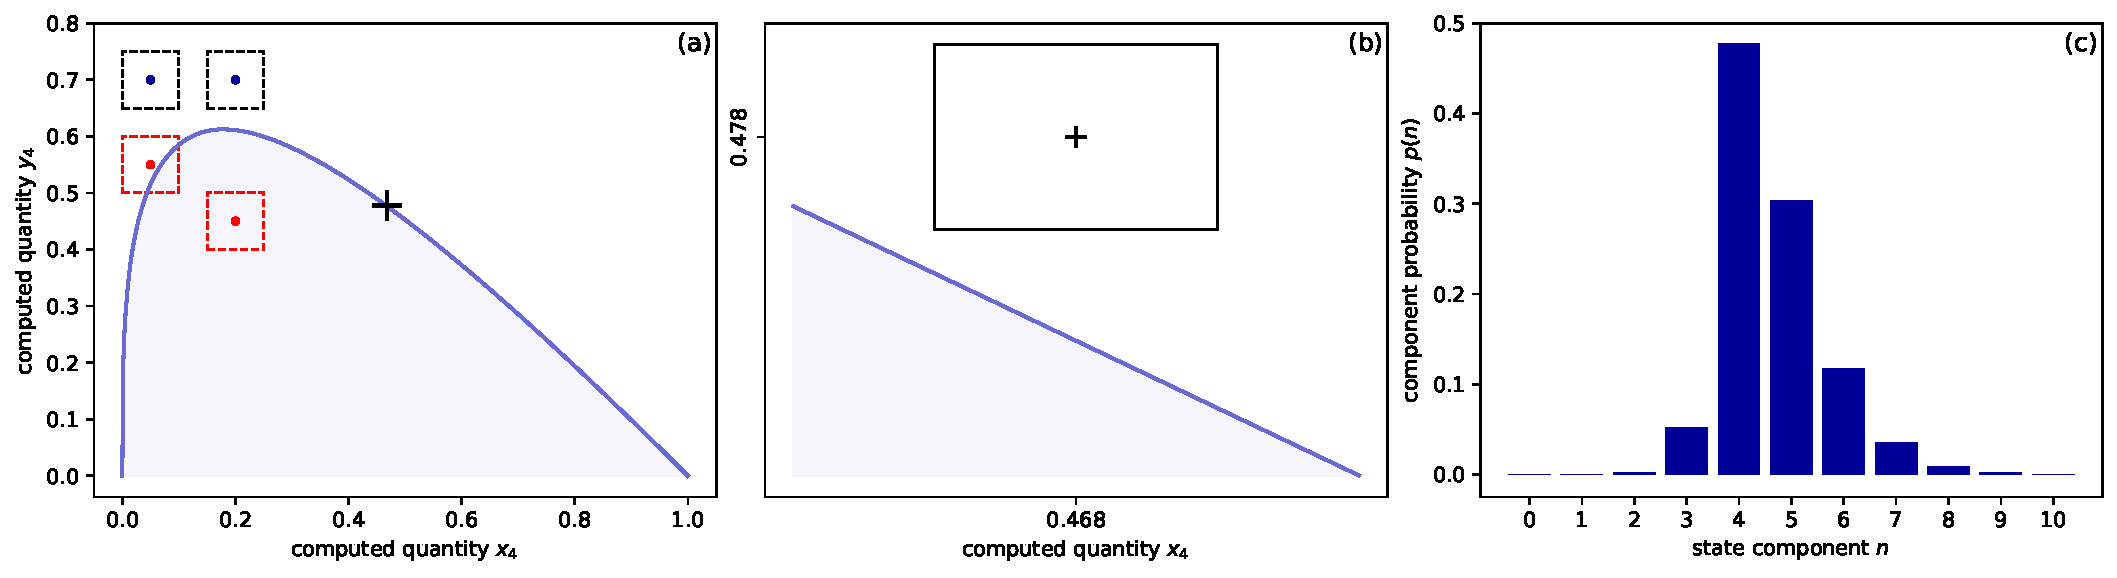
\includegraphics[width = 1.25 \columnwidth]{import/illustrate_process.pdf}
  \egroup
  \caption{
    Illustration of the certification procedure of genuine $4$-PQnG states for the simulated statistical ensembles. The blue line represents the threshold curve $F_{4} (x)$. States with $y_{4} > F_{4}(x_{4})$ are genuine $4$-PQnG states. Four example experimental states are depicted in the figure. The bullet points represent the expectation values obtained by simulating the experiment. The dashed boxes represent their uncertainty and span three standard deviations in both axial directions. The pictured boxes are exaggerated in size for the legibility of the illustration. States marked with red bullets failed the certification as they lie either under the threshold curve or their respective uncertainty boxes intersect the curve. States marked with blue bullets are certifiably genuine $4$-PQnG states according to the hierarchical criteria; their boxes are well above the curve and do not intersect the threshold curve.
  }
  \label{f-otm-il}
\end{figure}

% Monte Carlo Simulation
%

\subsection*{Monte Carlo simulation of the state preparation circuit}

The maximal tolerable amount of loss present in the optical circuit capable of preparing a certifiable genuine $m$-PQnG state can be determined by numerically simulating the experiment. The measurement statistics of a realistic experiment can be emulated using a Monte Carlo simulation based on the theoretical model of the circuit. The relations~\eqref{e-pnr-rho-kk}~and~\eqref{e-cap-rho-kk} determine the diagonal elements of the conditionally prepared quantum state depending on the choice of heralding detectors used in the experiment. Both relations are functions of the initial squeezing rate~$r$, the transmittances~$\zeta_{1}$ and~$\zeta_{2}$ of the lossy channels hindering both modes, and the post-selection criteria imposed on the measurement outcome $m$. The choice of the heralding detectors does not affect the simulation methodology and the subsequent state certification. The following description is therefore given in terms of the more straightforward relation~\eqref{e-pnr-rho-kk} derived for true PNR detectors.

The preparation circuit is evaluated for different amounts of loss in both modes, determined by the transmittances~$\zeta_{1}$ and~$\zeta_{2}$ with varying initial squeezing rates~$r$ and distinct target states~${m}$. Detection events in the simulated experiment are drawn as random samples from a multinomial distribution bootstrapped with the diagonal elements~$\braket{k|\hatrho_{(m)}|k}$ (where ${0 \leq k < 20}$) of the computed density matrix~\eqref{e-pnr-rho}. 

The number of random samples reflects the probability of successful preparation $P_{(m)}$. The probability~\eqref{e-pnr-pro} depends on the initial squeezing rate and the loss in the heralding mode. Given a budget of~$10^{8}$ repetitions available in a single realistic experimental run, only~${\lfloor 10^{8} \times P_{(m)} \rfloor}$ samples are drawn from the distribution and used to estimate the experimental probability distribution~${\overline{p}_{k} \approx \braket{k|\hatrho_{(m)}|k}}$. This random sampling process is repeated~$1000$ times to obtain an ensemble of independent experimental runs for the subsequent statistical analysis.

Certification of the simulated states is achieved with the hierarchical criteria~\cite{lachman2019}. The estimated experimental probabilities~$\overline{p}_{k}$, obtained in each simulated run of the experiment, are used to compute the aggregate random variables characterizing the experimental state,
%
\begin{equation}
  x_{m} = 1 - \sum_{k = 0}^{m} \overline{p}_{k} 
  \quad\text{and}\quad
  y_{m} = \overline{p}_{m} 
  \Qd
\end{equation}
%
Their expectation values and standard deviations, obtained from the ensemble of independent experimental runs, are then used to certify the quantum state resulting from the simulation with the particular choice of~${(m, \zeta_{1}, \zeta_{2}, r)}$ parameters. The experimental state is considered a certifiable genuine~$m$-PQnG state if the expectation values lie at least \textbf{three standard deviations} from the threshold function~$F_{m} (x)$ in both axial directions.

The operating principle of the certification procedure is illustrated in~\figref{f-otm-il}, with several example states shown, both passing and failing the certification, along with the actual threshold curve for genuine~$4$-PQnG states.

The extension of this methodology to include CAP detectors is mostly trivial. However, the infinite series in~\eqref{e-cap-pro} and~\eqref{e-cap-rho-kk} stemming from the expression~\eqref{e-cap} must be truncated accordingly. The number of elements considered in the series depends on the particular choice of the~$m$ and~$n$ parameters as these affect how the weight function~${w(i, m, n)}$ behaves. With~$m$ and~$n$ finite and close to each other, the weight function is generally heavy-tailed~\cite{provaznik2020}, and a sufficiently large cutoff for the summation has to be chosen.

% Results
%
%

\begin{figure}[h]
  \begin{center}
    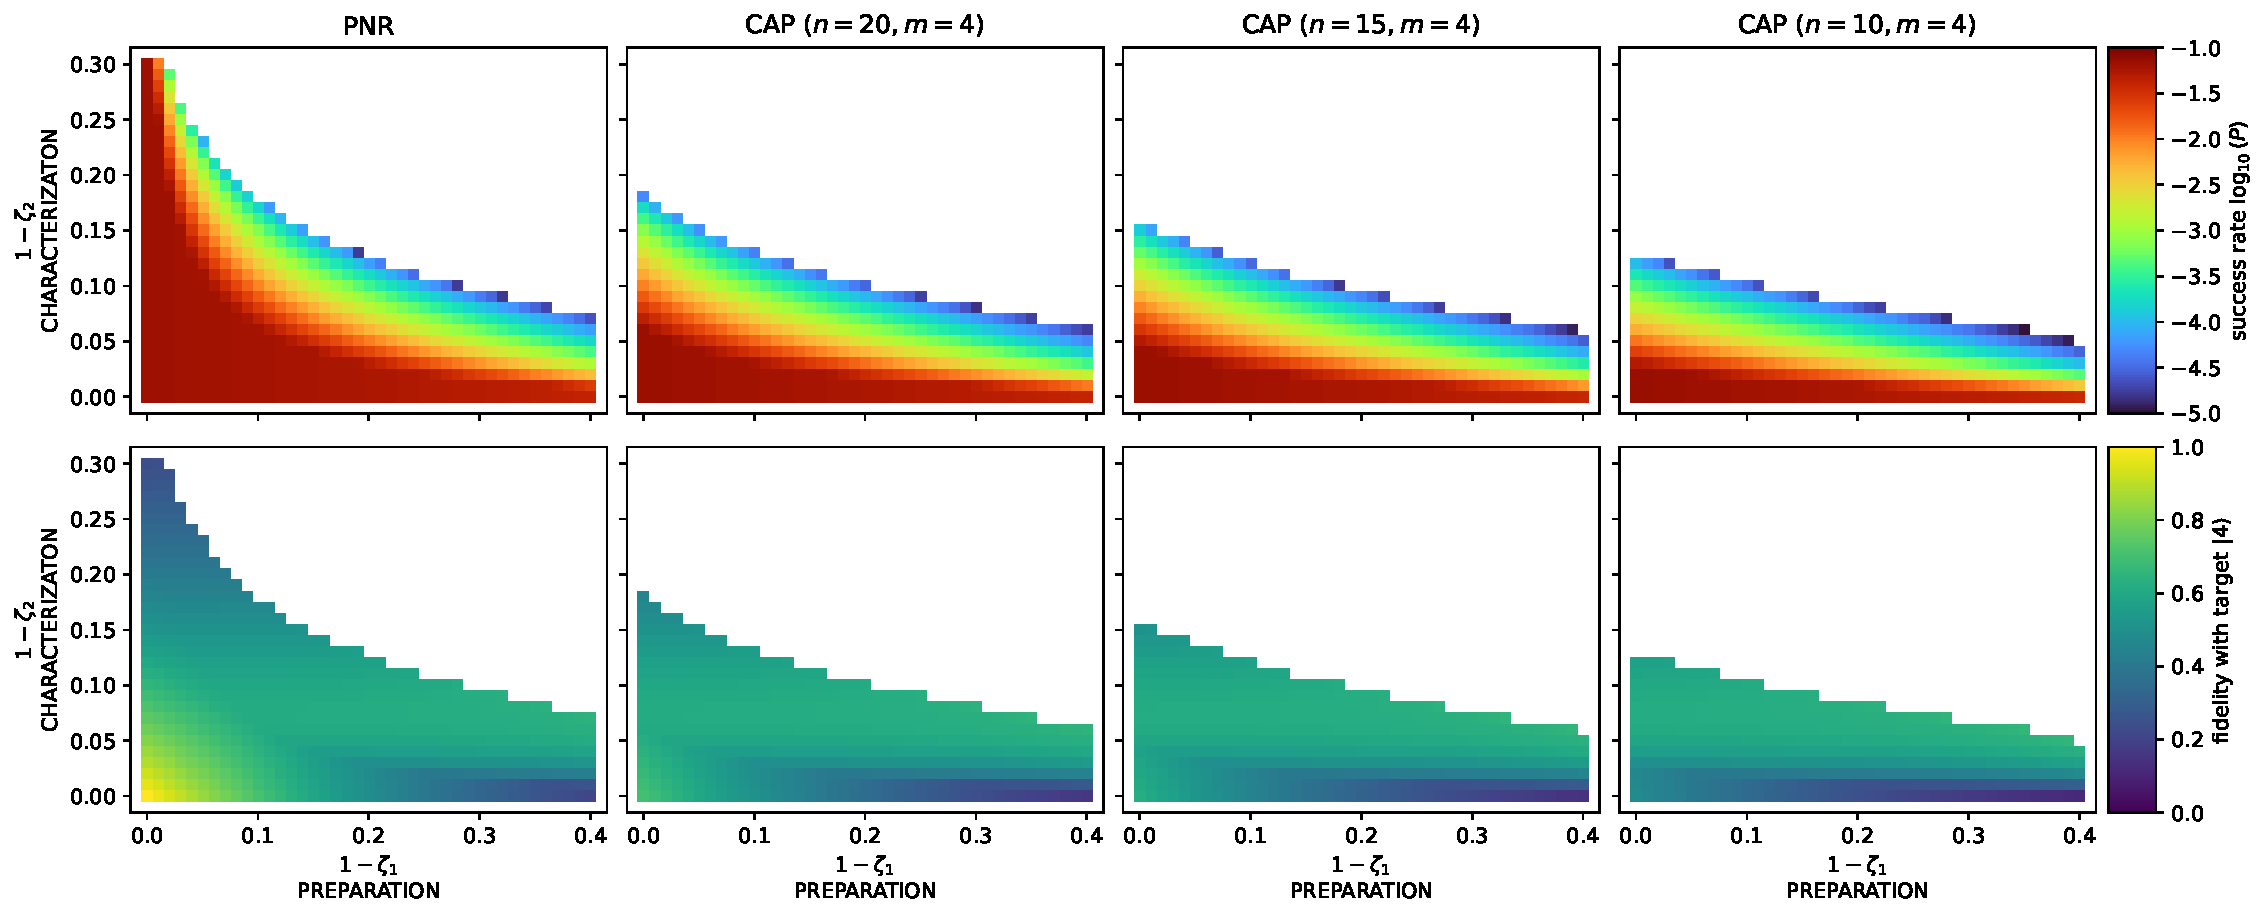
\includegraphics[width = \columnwidth]{import/202411/paper_unified_04.pdf}
  \end{center}
  \caption{
    The tolerable loss in preparation of certifiable genuine $4$-PQnG states. Individual tiles represent the best attainable probability of success (upper row) and the respective fidelity with the state of four photons (lower row). Values in each tile are obtained by maximizing the probability of successfully preparing a certifiable state over the initial squeezing rate~${0 \leq r \leq 10\dB}$. White tiles correspond to statistically insignificant cases with probabilities of success below $10^{-5}$. Different heralding detectors were used in the analysis. The results obtained for a true PNR detector are presented in the leftmost column, while the remaining columns represent CAP detectors with~${n = 20, 15}$, and~$10$ constituent avalanche detectors.
  }
  \label{f-res-4}
\end{figure}

\section{Discussion of results}

The main result of this work lies in finding out the maximal tolerable overall loss in the optical experiment for reliable production of certifiable genuine $4$-PQnG states. The use of the hierarchical criteria~\cite{lachman2019} is a necessity due to the realistic loss in preparation of the two-mode squeezed states used in the experiment, in their propagation, and the low detection efficiency of contemporary detectors with photon number resolving capacity, amplified by the practical unavailability of true PNR detectors. These issues affect the prepared states negatively, manifesting in suboptimal fidelities with the desired state and leading to poor interpretability of the results. Fidelity alone can not be reliably used to determine whether the prepared state is merely an attenuated state of four photons on something else entirely. Unlike fidelity, the hierarchical criteria, based on the stellar rank of the resulting state, offer concrete and unequivocal evidence of non-Gaussian behavior with a greater degree of robustness against loss~\cite{lachman2019}.

The results of the analysis of experimental preparation of certifiable genuine $4$-PQnG states are presented in \figref{f-res-4}. The analysis is done by considering different combinations of loss incurred during state preparation and its subsequent characterization. Certification of the prepared states accounts for realistic statistical behavior. The simulation reflects realistic experimental repetition rates. The cases with low probabilities of success (lower than~$10^{-5}$) leading to insufficient sample sizes below 1000 are excluded from the presented results. Values in each tile are obtained by maximizing the probability of successfully preparing of a certifiable state over the initial squeezing rate~${0 \leq r \leq 10\dB}$.

Experimental preparation of genuine $4$-PQnG states may just be feasible with state-of-the-art photon number resolving detectors~\cite{endo2021,endo2024}. Using alternative CAP detectors further increases the requirements  the experiment realization; however, the simulations suggest that experiments using cascades composed of sufficiently large numbers of high-quality avalanche detectors are also within the realm of feasibility. Notably, while the differences in probability of success between CAP and PNR detectors are significant, the differences between CAP detectors with $n = 10$ and $n = 20$ are not overwhelmingly significant.

\begin{figure}[h]
  \begin{center}
    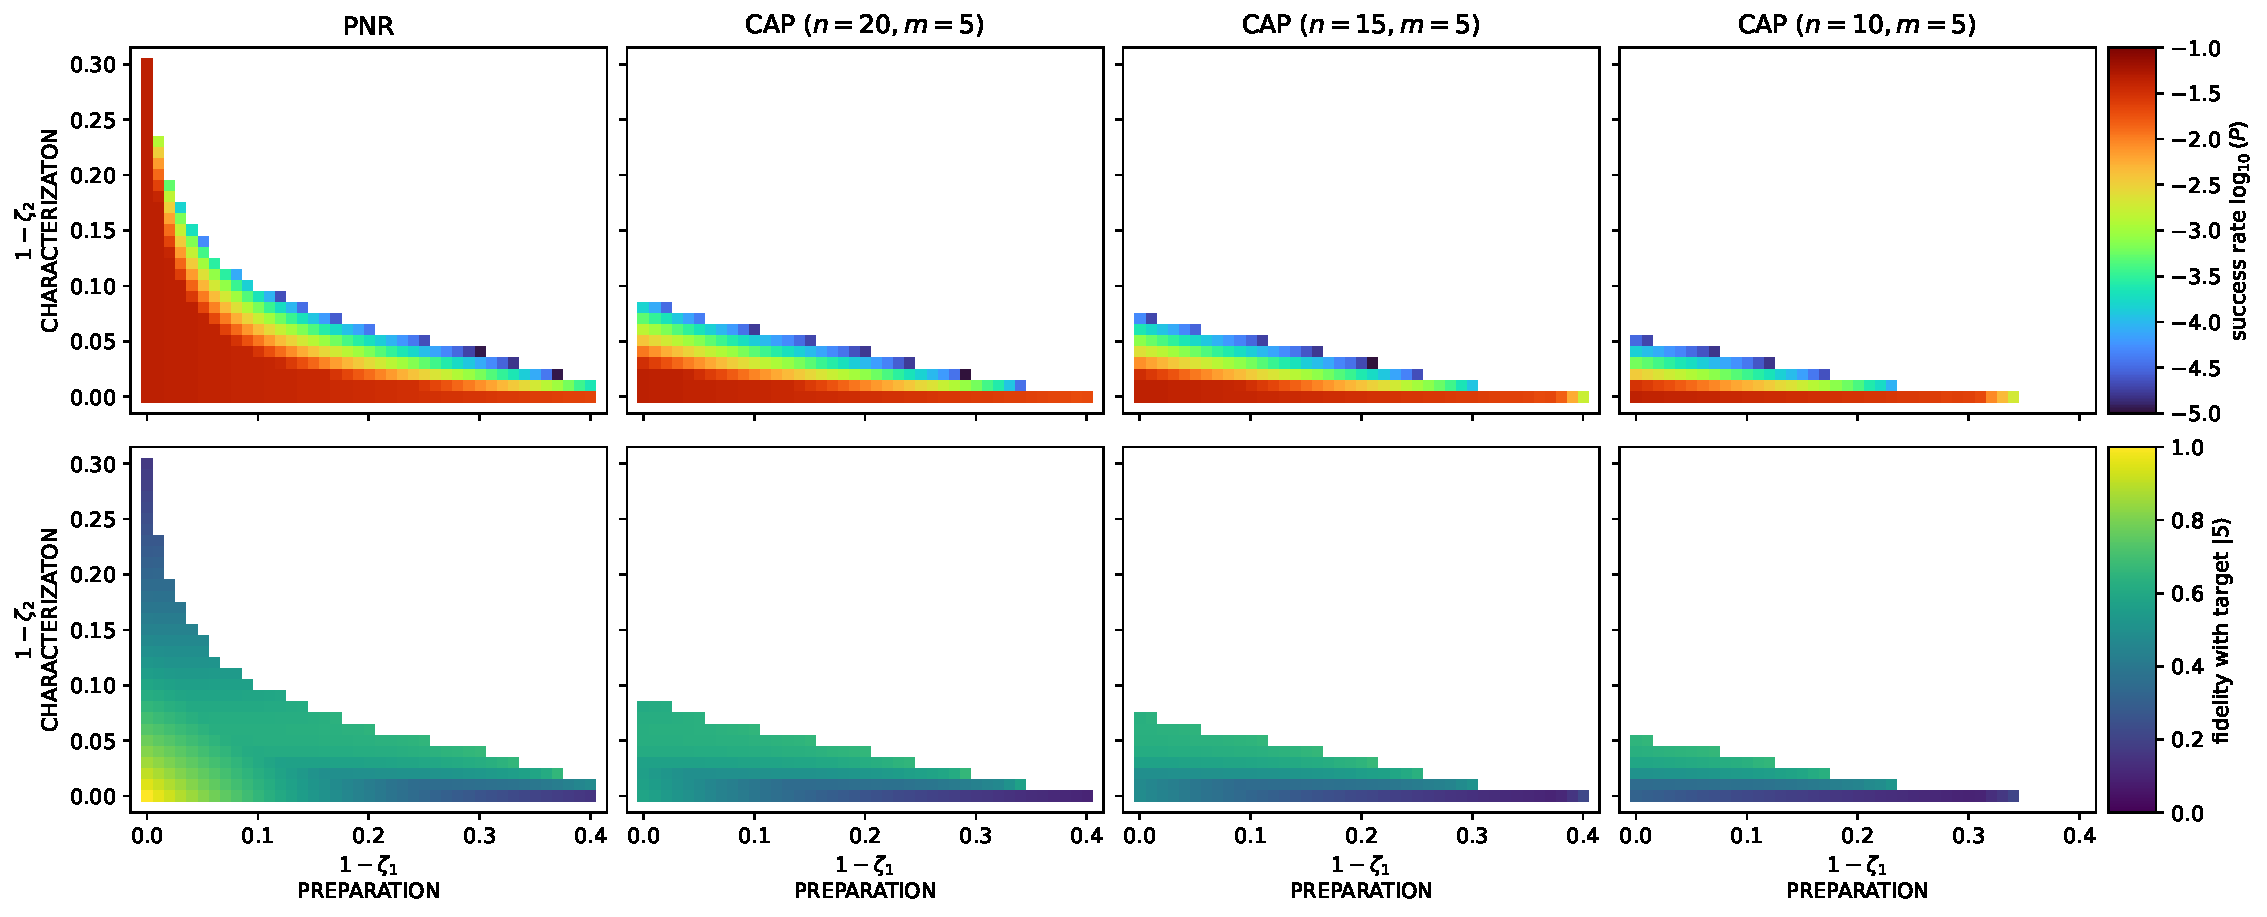
\includegraphics[width = \columnwidth]{import/202411/paper_unified_05.pdf}
  \end{center}
  \caption{
    The tolerable loss in preparation of certifiable genuine $5$-PQnG states. See \figref{f-res-4} for details.
  }
  \label{f-res-5}
\end{figure}

Furthermore, the analysis is extended to also include genuine $5$-PQnG states, as shown in \figref{f-res-5}. The overall difficulty of the experimental realization increases significantly, rendering the realization using CAP detectors with lower numbers (${n = 10, 15}$) of constituent detectors essentially infeasible. Even when using as many as $n = 20$ detectors, the feasible region is extremely narrow, allowing for at most $5\%$ of overall loss in its characterization while permitting non-zero loss during the preparation of the state.

This trend follows with states of higher order; this is only natural, as even in the ideal lossless case with a true PNR detector, the probability of success~\eqref{e-pnr-pro} scales with~${\lambda^{2m}}$ (where~${0 \leq \lambda < 1}$). Increasing the repetition rate in the analysis would balance the odds, as would increasing the number of detectors comprising the CAP detectors or using a true PNR detector.

We need to add the new set of plots revealing the boundaries.

% Conclusions
%

% \FloatBarrier
\section{Conclusions}

Well, motherfucker?

% References
%

\FloatBarrier
\printbibliography[heading = bibnumbered]

\end{document}

% vim: linebreak breakindent breakindentopt=shift\:-2 showbreak=↳\  syntax=tex colorcolumn=
